\documentclass[11pt,a4paper]{article}

\usepackage[T1]{fontenc}
\usepackage[utf8]{inputenc}
\usepackage[italian,provide=*]{babel}
\usepackage[margin=25mm]{geometry}
\usepackage{amsmath,amssymb}
\usepackage{siunitx}
\usepackage{booktabs}
\usepackage{tikz}
\usepackage{listings}
\usepackage{xcolor}
\usepackage{hyperref}
\usetikzlibrary{arrows.meta,positioning,calc}

\sisetup{detect-all,per-mode=symbol,exponent-product=\cdot}
\hypersetup{colorlinks=true,linkcolor=black,citecolor=black,urlcolor=blue!60!black}

\lstset{
  basicstyle=\ttfamily\footnotesize,
  keywordstyle=\bfseries,
  commentstyle=\itshape\color{gray!70!black},
  columns=fullflexible,
  breaklines=true,
  frame=single,
  framesep=4pt,
  rulecolor=\color{gray!50},
  morekeywords={component,nodes,parameters,variables,branches,equations,let,in,end,der,assert}
}

\newcommand{\opamp}{\texttt{opamp\_cfa}}

\title{\textbf{Modello Simscape di amplificatore\\ a retroazione di corrente (CFA)}\\[2mm]
\large Componente \opamp{} --- parametrizzazione LT1210}
\author{}
\date{}

\begin{document}
\maketitle
\vspace{-12mm}

\begin{abstract}
\noindent
Questo documento descrive il componente Simscape \opamp{}, un macromodello
comportamentale di amplificatore operazionale a retroazione di corrente
(\emph{current feedback amplifier}, CFA) con stadio d'uscita di potenza.
Vengono riportate le equazioni costitutive, le funzioni di regolarizzazione
usate per rendere il modello risolvibile da un solutore implicito, l'analisi
ad anello chiuso da cui discendono le relazioni di progetto dei parametri, e
la parametrizzazione sul dispositivo Analog Devices (ex Linear Technology)
LT1210, CFA da \SI{1.1}{\ampere} e \SI{35}{\mega\hertz}.
\end{abstract}

\section{Scopo e ambito}

Il modello nasce per simulare a livello di circuito stadi di pilotaggio ad
alta corrente (driver di cavo, pilotaggio di carichi capacitivi, stadi di
buffer per riferimenti di anelli di controllo) in cui il comportamento
dell'amplificatore non è idealizzabile: contano lo slew rate, il limite di
corrente, la saturazione rispetto alle alimentazioni e la dipendenza della
banda dalla rete di retroazione.

Il modello è \emph{comportamentale}: riproduce la funzione di trasferimento
ad anello aperto, i limiti di grande segnale e il bilancio energetico sui
pin di alimentazione, ma non deriva da una netlist a livello di transistor.
Non sono modellati distorsione armonica, rumore, CMRR e PSRR finiti,
dipendenza dalla temperatura, pin di \emph{shutdown} e di compensazione,
protezione termica.

\section{Richiamo: CFA contro VFA}

In un amplificatore a retroazione di tensione (VFA) l'ingresso è una coppia
differenziale ad alta impedenza e il guadagno ad anello aperto è
$A(s)\simeq A_0/(1+s/\omega_p)$, con prodotto guadagno--banda costante: la
banda ad anello chiuso scala con l'inverso del guadagno.

In un CFA l'ingresso non invertente pilota un \emph{buffer di tensione} la
cui uscita è il morsetto invertente. Il morsetto invertente è quindi a bassa
impedenza (resistenza serie $R_{\mathrm{inv}}$, tipicamente qualche
\si{\ohm}) e la grandezza d'errore non è una tensione differenziale ma la
corrente $i_{\mathrm{err}}$ che il buffer eroga. Tale corrente viene
specchiata su un nodo ad alta impedenza, la cui impedenza di transimpedenza
$Z(s)$ genera la tensione d'uscita:
\begin{equation}
  v_{o} = Z(s)\, i_{\mathrm{err}},
  \qquad
  Z(s) = \frac{R_t}{1+s R_t C_t}.
\end{equation}
Poiché il guadagno d'anello vale $T(s)=Z(s)/R_f$, la banda ad anello chiuso
dipende dal solo resistore di retroazione e non dal guadagno: è la proprietà
caratteristica del CFA, e insieme all'assenza di limitazione di slew da
corrente di coda spiega gli slew rate di
\SIrange{800}{1100}{\volt\per\micro\second} tipici di questi dispositivi.
Il rovescio della medaglia è che $R_f$ non è libero: valori troppo bassi
riducono il margine di fase fino all'oscillazione, e non si può porre una
capacità in parallelo a $R_f$~\cite{ltdatasheet,franco}.

\section{Architettura del macromodello}

\begin{figure}[h]
\centering
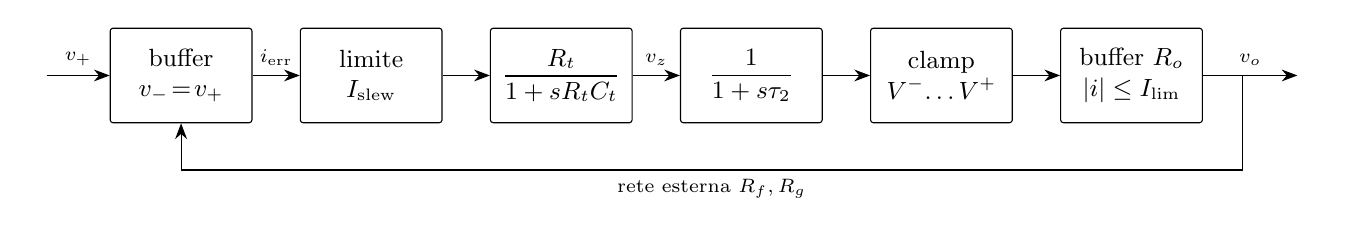
\begin{tikzpicture}[
  node distance=6mm,
  blk/.style={draw,rounded corners=1pt,minimum height=12mm,minimum width=18mm,align=center,font=\small},
  >={Stealth[length=2mm]}
]
\node (in) at (0,0) {};
\node[blk,right=8mm of in] (buf) {buffer\\ $v_-\!=\!v_+$};
\node[blk,right=of buf] (mir) {limite\\ $I_{\mathrm{slew}}$};
\node[blk,right=of mir] (z)   {$\dfrac{R_t}{1+sR_tC_t}$};
\node[blk,right=of z]  (p2)   {$\dfrac{1}{1+s\tau_2}$};
\node[blk,right=of p2] (clip) {clamp\\ $V^-\!\ldots V^+$};
\node[blk,right=of clip] (ob) {buffer $R_o$\\ $|i|\le I_{\mathrm{lim}}$};
\node[right=12mm of ob] (out) {};

\draw[->] (in) -- node[above,font=\scriptsize]{$v_+$} (buf);
\draw[->] (buf) -- node[above,font=\scriptsize]{$i_{\mathrm{err}}$} (mir);
\draw[->] (mir) -- (z);
\draw[->] (z) -- node[above,font=\scriptsize]{$v_z$} (p2);
\draw[->] (p2) -- (clip);
\draw[->] (clip) -- (ob);
\draw[->] (ob) -- node[above,font=\scriptsize]{$v_o$} (out);

\coordinate (fbdown) at ($(ob.east)+(5mm,0)$);
\draw[->] (fbdown) -- ++(0,-12mm) -| node[pos=0.25,below,font=\scriptsize]{rete esterna $R_f,R_g$} ($(buf.south)+(0mm,0)$);
\end{tikzpicture}

\caption{Catena diretta del macromodello. Il morsetto invertente coincide
con l'uscita del buffer d'ingresso; la retroazione è chiusa esternamente
dalla rete $R_f$--$R_g$ collegata a tale morsetto.}
\end{figure}

Il componente espone cinque nodi elettrici: i due ingressi \texttt{p} e
\texttt{m}, l'uscita \texttt{out} e i due nodi di alimentazione
\texttt{vsp} e \texttt{vsn}. I nodi di alimentazione non sono decorativi:
le equazioni impongono il bilancio esatto delle correnti, quindi la potenza
assorbita dagli alimentatori e la dissipazione del dispositivo sono
coerenti, e un'alimentazione con impedenza non nulla produce la riduzione
di escursione d'uscita che si osserva in pratica.

\section{Equazioni costitutive}

Si adotta la convenzione di Simscape: per ogni nodo la corrente di ramo è
positiva se entra nel componente. Sono variabili del modello
$i_p, i_m, i_o, i_{sp}, i_{sn}$ e gli stati interni $v_c$, $v_z$, $v_2$.

\subsection{Stadio d'ingresso}

Il morsetto non invertente presenta la corrente di polarizzazione $I_{b+}$,
la resistenza di modo comune $R_{\mathrm{in}+}$ e la capacità
$C_{\mathrm{in}+}$:
\begin{equation}
  v_c = v_p,
  \qquad
  i_p = I_{b+} + \frac{v_c}{R_{\mathrm{in}+}} + C_{\mathrm{in}+}\,\dot v_c .
\end{equation}

La tensione d'ingresso viene limitata alla finestra di modo comune
ammessa, $v_{p,e}=\mathrm{sat}(v_p)$ fra $v_{sn}+V_{cm-}$ e
$v_{sp}-V_{cm+}$ (la saturazione regolarizzata è definita nella
sezione~\ref{sec:smooth}). Il buffer d'ingresso, con offset $V_{os}$ e
resistenza serie $R_{\mathrm{inv}}$, impone
\begin{equation}
  v_m = v_{p,e} + V_{os} + R_{\mathrm{inv}}\, i_m .
  \label{eq:buffer}
\end{equation}
La corrente d'errore è quella \emph{uscente} dal morsetto invertente, al
netto della corrente di polarizzazione $I_{b-}$:
\begin{equation}
  i_{\mathrm{err}} = -\left(i_m - I_{b-}\right).
  \label{eq:ierr}
\end{equation}
Il segno è quello fisico: iniettando corrente nel morsetto invertente
($i_m>0$, come in un amplificatore a transimpedenza pilotato da fotodiodo)
l'uscita va in negativo.

\subsection{Nodo di transimpedenza e limite di slew}

La corrente d'errore viene trasferita al nodo ad alta impedenza dallo
specchio di corrente, che satura. La saturazione è resa continua con una
tangente iperbolica:
\begin{equation}
  i_{\mathrm{lim}} = I_{\mathrm{slew}} \tanh\!\left(\frac{i_{\mathrm{err}}}{I_{\mathrm{slew}}}\right),
  \qquad
  C_t\,\dot v_z = i_{\mathrm{lim}} - \frac{v_z}{R_t}.
  \label{eq:tz}
\end{equation}
Il limite $I_{\mathrm{slew}}$ sulla corrente che carica $C_t$ è ciò che
produce il limite di slew rate:
\begin{equation}
  \mathrm{SR} = \frac{I_{\mathrm{slew}}}{C_t}.
  \label{eq:sr}
\end{equation}

\subsection{Polo parassita}

Un ritardo del primo ordine rappresenta il polo dello stadio d'uscita, che
è responsabile del picco di risposta e del roll-off oltre la frequenza di
attraversamento:
\begin{equation}
  \tau_2\,\dot v_2 = v_z - v_2,
  \qquad \tau_2 = \frac{1}{2\pi f_{p2}}.
\end{equation}

\subsection{Stadio d'uscita}

La tensione $v_2$ viene limitata alla finestra ammessa rispetto ai nodi di
alimentazione,
\begin{equation}
  v_{o,\mathrm{id}} = \mathrm{sat}\left(v_2;\; v_{sn}+V_{\mathrm{sat}-},\; v_{sp}-V_{\mathrm{sat}+}\right),
\end{equation}
e il buffer d'uscita eroga una corrente con pendenza $1/R_o$ attorno
all'origine e limite $I_{\mathrm{lim}}$:
\begin{equation}
  x_o = \frac{v_{o,\mathrm{id}} - v_{\mathrm{out}}}{R_o I_{\mathrm{lim}}},
  \qquad
  i_{\mathrm{load}} = -i_o = I_{\mathrm{lim}}\,\frac{x_o}{\left(1+x_o^{4}\right)^{1/4}} .
  \label{eq:iout}
\end{equation}
Per $|x_o|\ll 1$ si ha $i_{\mathrm{load}}\simeq (v_{o,\mathrm{id}}-v_{\mathrm{out}})/R_o$,
cioè un generatore di tensione con resistenza serie $R_o$; per
$|x_o|\to\infty$ la corrente tende a $\pm I_{\mathrm{lim}}$.

\subsection{Alimentazioni}

La corrente di carico va ripartita fra i due rail in funzione del suo
segno. La ripartizione è resa continua con
\begin{equation}
  i_{\mathrm{pos}} = \tfrac{1}{2}\left(i_{\mathrm{load}} + \sqrt{i_{\mathrm{load}}^{2}+\delta_I^{2}}\right)
  \;\simeq\; \max(i_{\mathrm{load}},0),
  \qquad
  i_{\mathrm{neg}} = i_{\mathrm{load}} - i_{\mathrm{pos}},
\end{equation}
da cui
\begin{equation}
  i_{sp} = I_q + i_{\mathrm{pos}},
  \qquad
  i_{sn} = -I_q + i_{\mathrm{neg}} - i_p - i_m .
\end{equation}
Gli ultimi due termini garantiscono $i_p+i_m+i_o+i_{sp}+i_{sn}=0$, cioè
nessuna corrente spuria verso il nodo di riferimento. La dissipazione
istantanea del dispositivo è quindi
\begin{equation}
  p_{\mathrm{diss}} = v_{sp} i_{sp} + v_{sn} i_{sn} + v_{\mathrm{out}} i_o
  + v_p i_p + v_m i_m .
\end{equation}

\section{Funzioni di regolarizzazione}
\label{sec:smooth}

Simscape risolve un sistema DAE implicito con solutori che richiedono
Jacobiani continui: discontinuità o derivate non continue nelle equazioni
producono passi rifiutati, eventi ripetuti e, in casi sfavorevoli, mancata
convergenza. Tutti i limiti del modello sono quindi espressi con funzioni
$C^{\infty}$.

\paragraph{Saturazione.} Il minimo e il massimo regolarizzati sono
\begin{equation}
  \mathrm{smin}_\delta(a,b) = \tfrac{1}{2}\left(a+b-\sqrt{(a-b)^2+\delta^2}\right),
  \qquad
  \mathrm{smax}_\delta(a,b) = \tfrac{1}{2}\left(a+b+\sqrt{(a-b)^2+\delta^2}\right),
\end{equation}
e $\mathrm{sat}(x;l,h)=\mathrm{smax}_\delta\!\left(\mathrm{smin}_\delta(x,h),l\right)$.
Lo sviluppo di $\sqrt{(a-b)^2+\delta^2}$ per $|a-b|\gg\delta$ dà
\begin{equation}
  \mathrm{smin}_\delta(a,b) \simeq \min(a,b) - \frac{\delta^{2}}{4|a-b|},
\end{equation}
quindi l'errore lontano dal ginocchio è del secondo ordine in $\delta$: con
$\delta=\SI{100}{\milli\volt}$ e una distanza dal rail di \SI{13}{\volt}
l'errore è inferiore a \SI{0.2}{\milli\volt}, trascurabile rispetto a
$V_{os}$. Il costo è che la saturazione ha un ginocchio arrotondato su una
larghezza $\sim\delta$.

\paragraph{Limitatore di corrente.} La forma
$x/(1+x^{4})^{1/4}$ usata nella~\eqref{eq:iout} ha ginocchio più netto della
tangente iperbolica a parità di pendenza iniziale e di asintoto
($0{,}841\,I_{\mathrm{lim}}$ contro $0{,}762\,I_{\mathrm{lim}}$ in $x=1$),
resta dispari e ha derivata continua ovunque. Nel codice si scrive come
\texttt{sqrt(sqrt(1+xo\^{}4))} per evitare l'elevamento a potenza frazionaria.

\section{Analisi ad anello chiuso}

\subsection{Guadagno e banda}

Si consideri la configurazione non invertente con $R_f$ fra uscita e
morsetto invertente e $R_g$ fra morsetto invertente e massa; sia
$G = 1 + R_f/R_g$ il guadagno di rumore. Dalla~\eqref{eq:buffer}, con
$i_m=-i_{\mathrm{err}}$ e trascurando le correnti di polarizzazione,
\begin{equation}
  v_m = v_{\mathrm{in}} - R_{\mathrm{inv}} i_{\mathrm{err}},
  \qquad
  i_{\mathrm{err}} = \frac{v_m}{R_g} + \frac{v_m - v_o}{R_f}
                   = \frac{G}{R_f} v_m - \frac{v_o}{R_f}.
\end{equation}
Sostituendo e usando $v_o = Z(s)\,i_{\mathrm{err}}$ si ottiene
\begin{equation}
  \boxed{\;
  A(s) = \frac{v_o}{v_{\mathrm{in}}}
       = \frac{G}{1 + \dfrac{R_{\mathrm{eff}}}{Z(s)}},
  \qquad
  R_{\mathrm{eff}} = R_f + G\,R_{\mathrm{inv}} \; }
  \label{eq:cl}
\end{equation}
Il risultato è quello noto per i CFA: la resistenza di retroazione
\emph{efficace} è $R_f$ maggiorata di $G\,R_{\mathrm{inv}}$, ed è per questo
che la banda, pur essendo in prima approssimazione indipendente dal
guadagno, si riduce leggermente ai guadagni elevati.

L'errore di guadagno in continua vale
\begin{equation}
  \frac{A(0)}{G} = \frac{1}{1 + R_{\mathrm{eff}}/R_t} \simeq 1 - \frac{R_{\mathrm{eff}}}{R_t},
\end{equation}
cioè circa lo \SI{0.3}{\percent} con i valori di tabella: il valore finito
della transimpedenza $R_t$, non il guadagno di tensione, è il parametro che
fissa la precisione statica di un CFA.

\subsection{Frequenza di attraversamento, \texorpdfstring{$Q$}{Q} e picco}

Con $R_t\to\infty$ e includendo il polo parassita, il denominatore
della~\eqref{eq:cl} diventa
\begin{equation}
  1 + \frac{s}{\omega_t} + \frac{\tau_2}{\omega_t}s^{2},
  \qquad
  \omega_t = \frac{1}{R_{\mathrm{eff}} C_t},
\end{equation}
cioè un sistema del secondo ordine con
\begin{equation}
  \boxed{\;
  f_0 = \sqrt{f_t\,f_{p2}},
  \qquad
  Q = \sqrt{\frac{f_t}{f_{p2}}},
  \qquad
  f_t = \frac{1}{2\pi R_{\mathrm{eff}} C_t}\;}
  \label{eq:Q}
\end{equation}
Il picco di risposta è $1/\left(2\zeta\sqrt{1-\zeta^{2}}\right)$ con
$\zeta=1/(2Q)$, e la banda a \SI{-3}{\decibel} è
\begin{equation}
  f_{-3\mathrm{dB}} = f_0\sqrt{\,1-\tfrac{1}{2Q^{2}} + \sqrt{\left(1-\tfrac{1}{2Q^{2}}\right)^{2}+1}\,}.
  \label{eq:f3}
\end{equation}

È un punto da tenere presente in fase di parametrizzazione: la banda a
\SI{-3}{\decibel} \textbf{non} coincide con $f_t$. Per $Q\simeq 1$ vale
$f_{-3\mathrm{dB}}\simeq 1{,}3\,f_t$, e senza polo parassita
($f_{p2}\to\infty$) si ricadrebbe su $f_{-3\mathrm{dB}}=f_t$. I costruttori
dichiarano la banda in condizioni di picco $\le\SI{1}{\decibel}$, quindi
$f_t$ va scelto \emph{sotto} il valore di banda dichiarato. Alcuni valori
utili:

\begin{table}[h]
\centering
\begin{tabular}{cccc}
\toprule
$f_{p2}/f_t$ & $Q$ & picco (\si{\decibel}) & $f_{-3\mathrm{dB}}/f_t$ \\
\midrule
$\infty$ & --    & 0{,}00 & 1{,}00 \\
4{,}0    & 0{,}50 & 0{,}00 & 1{,}13 \\
2{,}0    & 0{,}71 & 0{,}00 & 1{,}27 \\
1{,}1    & 0{,}95 & 0{,}97 & 1{,}30 \\
1{,}0    & 1{,}00 & 1{,}25 & 1{,}27 \\
0{,}5    & 1{,}41 & 3{,}01 & 1{,}10 \\
\bottomrule
\end{tabular}
\caption{Effetto del polo parassita, dalle~\eqref{eq:Q} e~\eqref{eq:f3}.}
\end{table}

\subsection{Relazioni di progetto dei parametri}

I due parametri interni $C_t$ e $I_{\mathrm{slew}}$ non si dichiarano
direttamente ma si ricavano da grandezze di catalogo, tramite le
\eqref{eq:Q} e~\eqref{eq:sr}:
\begin{equation}
  C_t = \frac{1}{2\pi f_t R_{f,\mathrm{nom}}},
  \qquad
  I_{\mathrm{slew}} = \mathrm{SR}\cdot C_t .
\end{equation}
Dichiarando $f_t$ alla resistenza di retroazione nominale
$R_{f,\mathrm{nom}}$, il modello riproduce automaticamente la dipendenza
della banda da $R_f$ e la sua quasi indipendenza dal guadagno, che è il
comportamento distintivo del CFA.

\subsection{Slew rate}

Nel modello lo slew rate è costante e pari a $I_{\mathrm{slew}}/C_t$. Nel
dispositivo reale dipende invece dalla configurazione, perché concorrono
sia il limite dello stadio d'ingresso (legato alla corrente di riposo) sia
quello dello stadio d'uscita (legato a $R_f$): per l'LT1210 si passa da
circa \SI{770}{\volt\per\micro\second} a guadagno $+1$ a circa
\SI{1100}{\volt\per\micro\second} a guadagno $-1$~\cite{ltdatasheet}. Il
modello va quindi tarato sulla configurazione d'interesse.

Un secondo meccanismo di limitazione è invece riprodotto correttamente:
con carico capacitivo la velocità è limitata dalla corrente d'uscita,
$\mathrm{d}v/\mathrm{d}t = I_{\mathrm{lim}}/C_L$. Con
$C_L = \SI{10}{\nano\farad}$ e $I_{\mathrm{lim}}=\SI{1.5}{\ampere}$ si
ottengono \SI{150}{\volt\per\micro\second}, in accordo con il datasheet.

\section{Parametrizzazione LT1210}

L'LT1210 è un CFA da \SI{1.1}{\ampere} di corrente d'uscita minima,
alimentabile fra \SI{\pm5}{\volt} e \SI{\pm15}{\volt}, stabile su carichi
capacitivi fino a \SI{10}{\nano\farad}. I valori di
tabella~\ref{tab:par} sono i tipici a \SI{\pm15}{\volt} e \SI{25}{\celsius}.

\begin{table}[h]
\centering
\small
\begin{tabular}{llll}
\toprule
Parametro & Valore & Grandezza & Origine \\
\midrule
\texttt{Rt}      & \SI{260}{\kilo\ohm}  & transimpedenza c.c. $R_t$ & datasheet, tip. (min \SI{100}{\kilo\ohm}) \\
\texttt{f\_t}    & \SI{42}{\mega\hertz} & attraversamento con $R_{f,\mathrm{nom}}$ & fit sulla tabella AC \\
\texttt{Rf\_nom} & \SI{680}{\ohm}       & $R_f$ di riferimento & datasheet, condizione di banda \\
\texttt{f\_p2}   & \SI{46}{\mega\hertz} & polo parassita & fit sul picco $\le\SI{1}{\decibel}$ \\
\texttt{SR}      & \SI{900}{\volt\per\micro\second} & slew rate & datasheet, $A_V=2$ \\
\midrule
\texttt{Rinv}    & \SI{15}{\ohm}        & resistenza d'ingresso invertente & \textbf{stimato} (non specificato) \\
\texttt{Vos}     & \SI{3}{\milli\volt}  & offset d'ingresso & datasheet, tip. (max \SI{15}{\milli\volt}) \\
\texttt{Ib\_p}   & \SI{2}{\micro\ampere}  & corrente di polarizzazione $+$ & datasheet, tip. \\
\texttt{Ib\_m}   & \SI{10}{\micro\ampere} & corrente di polarizzazione $-$ & datasheet, tip. \\
\texttt{Rin\_p}  & \SI{10}{\mega\ohm}   & resistenza d'ingresso $+$ & datasheet, tip. \\
\texttt{Cin\_p}  & \SI{2}{\pico\farad}  & capacità d'ingresso $+$ & datasheet \\
\texttt{Vcm\_p/n}& \SI{1.5}{\volt}      & margine di modo comune & da $\pm\SI{13.5}{\volt}$ tip. \\
\midrule
\texttt{Ro}      & \SI{1.5}{\ohm}       & resistenza d'uscita ad anello aperto & \textbf{ricavato} (vedi sotto) \\
\texttt{Vsat\_p/n}& \SI{1.8}{\volt}     & tensione di saturazione a vuoto & \textbf{ricavato} (vedi sotto) \\
\texttt{Ilim}    & \SI{1.5}{\ampere}    & limite di corrente & nota applicativa su $C_L$ \\
\texttt{Iq}      & \SI{35}{\milli\ampere} & corrente di riposo & datasheet, tip. \\
\midrule
\texttt{dV}      & \SI{0.1}{\volt}      & regolarizzazione dei clamp & numerico \\
\texttt{dI}      & \SI{1}{\milli\ampere}& regolarizzazione della ripartizione & numerico \\
\bottomrule
\end{tabular}
\caption{Parametri di default del componente \opamp{}.}
\label{tab:par}
\end{table}

\paragraph{Stadio d'uscita.} Il datasheet dichiara un'escursione tipica di
$\pm\SI{11.5}{\volt}$ su $R_L=\SI{10}{\ohm}$ con
$V_S=\SI{\pm15}{\volt}$, cioè \SI{1.15}{\ampere}, mentre la curva di
tensione di saturazione a carico leggero dà circa \SI{1.8}{\volt}. Da qui
\begin{equation}
  R_o = \frac{(15 - 1{,}8) - 11{,}5}{1{,}15} \approx \SI{1.5}{\ohm},
\end{equation}
che si riconduce alla resistenza d'uscita ad anello aperto: ad anello
chiuso viene divisa per il guadagno d'anello e non è direttamente
osservabile.

\paragraph{Dinamica.} $f_t$ e $f_{p2}$ sono stati ricavati imponendo
banda \SI{55}{\mega\hertz} e picco $\simeq\SI{1}{\decibel}$ con
$R_f=R_g=\SI{680}{\ohm}$, secondo le~\eqref{eq:Q} e~\eqref{eq:f3}. Ne
discende $C_t=\SI{5.6}{\pico\farad}$ e
$I_{\mathrm{slew}}=\SI{5.0}{\milli\ampere}$. Il confronto con la tabella
delle prestazioni AC del datasheet è riportato in
tabella~\ref{tab:valid}.

\begin{table}[h]
\centering
\small
\begin{tabular}{llccc}
\toprule
Configurazione & $R_f$ & datasheet & modello & picco modello \\
\midrule
$A_V=+1$, $R_L=\SI{150}{\ohm}$  & \SI{750}{\ohm} & \SI{56.8}{\mega\hertz} & \SI{50.0}{\mega\hertz} & \SI{0.7}{\decibel} \\
$A_V=+2$, $R_L=\SI{150}{\ohm}$  & \SI{665}{\ohm} & \SI{52.5}{\mega\hertz} & \SI{53.8}{\mega\hertz} & \SI{0.9}{\decibel} \\
$A_V=-1$, $R_L=\SI{150}{\ohm}$  & \SI{604}{\ohm} & \SI{66.2}{\mega\hertz} & \SI{57.6}{\mega\hertz} & \SI{1.2}{\decibel} \\
$A_V=+10$, $R_L=\SI{150}{\ohm}$ & \SI{453}{\ohm} & \SI{61.5}{\mega\hertz} & \SI{59.8}{\mega\hertz} & \SI{1.3}{\decibel} \\
\bottomrule
\end{tabular}
\caption{Banda a \SI{-3}{\decibel}: confronto fra tabella AC del datasheet
($V_S=\SI{\pm15}{\volt}$, $I_S=\SI{35}{\milli\ampere}$) e
modello~\eqref{eq:cl}. Lo scarto resta entro il \SI{13}{\percent}.}
\label{tab:valid}
\end{table}

Il modello non riproduce la riduzione di banda con carichi resistivi
pesanti (a $R_L=\SI{10}{\ohm}$ il dispositivo reale scende a
\SI{35}{\mega\hertz}), perché $f_{p2}$ è fisso e indipendente dal carico.
Per simulare quella condizione va abbassato $f_{p2}$.

\section{Procedura di verifica}

\begin{enumerate}
\item \textbf{Continua.} Montaggio non invertente $G=2$
  ($R_f=R_g=\SI{680}{\ohm}$), ingresso a rampa lenta: verificare l'offset
  d'uscita ($G\,V_{os}$), l'errore di guadagno e le soglie di saturazione a
  $\pm(V_S - V_{\mathrm{sat}} - R_o i_L)$.
\item \textbf{Piccolo segnale.} Analisi in frequenza (linearizzazione o
  sweep sinusoidale a \SI{10}{\milli\volt}) con $R_L=\SI{100}{\ohm}$:
  attesi \SI{53}{\mega\hertz} e picco inferiore a \SI{1}{\decibel}.
\item \textbf{Firma del CFA.} Ripetere con $R_f=\SI{1.5}{\kilo\ohm}$ a
  guadagno invariato: la banda deve circa dimezzarsi. Ripetere poi con
  $G=10$ e $R_f$ invariato: la banda deve restare quasi la stessa.
\item \textbf{Slew rate.} Gradino d'ingresso da \SI{5}{\volt} su
  $R_L=\SI{400}{\ohm}$: attesi \SI{900}{\volt\per\micro\second}.
\item \textbf{Limite di corrente.} Carico $C_L=\SI{10}{\nano\farad}$: la
  pendenza d'uscita deve saturare a $I_{\mathrm{lim}}/C_L =
  \SI{150}{\volt\per\micro\second}$.
\item \textbf{Bilancio di potenza.} Con alimentatori ideali verificare
  $\sum i = 0$ sui cinque nodi e la coerenza fra potenza assorbita, potenza
  sul carico e dissipazione.
\end{enumerate}

\section{Limiti del modello}

\begin{itemize}
\item Slew rate costante, non dipendente da configurazione e corrente di
  riposo.
\item $f_{p2}$ indipendente dal carico: la banda non si riduce sui carichi
  resistivi bassi.
\item Nessuna capacità parassita sul nodo invertente: il picco di risposta
  che ne deriva va introdotto aggiungendo esternamente un condensatore su
  quel nodo.
\item Nessun pin di \emph{shutdown}, nessun pin di compensazione, nessuna
  protezione termica, nessuna dipendenza dalla temperatura.
\item CMRR e PSRR infiniti, rumore e distorsione assenti.
\item Il limite di corrente è la corrente di picco utile, non la corrente
  di cortocircuito (superiore, e comunque limitata termicamente).
\item I clamp regolarizzati hanno un ginocchio di larghezza $\sim\delta$:
  valori di $\delta$ troppo grandi falsano la saturazione, valori troppo
  piccoli rallentano il solutore.
\end{itemize}

\section{Interfaccia del componente}

\begin{lstlisting}
component opamp_cfa
  nodes
    p, m          % ingressi non invertente e invertente
    vsp, vsn      % alimentazioni
    out           % uscita
  variables
    i_p, i_m, i_o, i_sp, i_sn   % correnti di ramo
    vc                          % tensione su Cin_p
    vz                          % nodo di transimpedenza
    v2                          % uscita del polo parassita
\end{lstlisting}

Gli stati dinamici sono tre ($v_c$, $v_z$, $v_2$); ponendo
$C_{\mathrm{in}+}=0$ la prima equazione degenera in un vincolo algebrico e
lo stato corrispondente scompare.

\begin{thebibliography}{9}

\bibitem{ltdatasheet}
Analog Devices, \emph{LT1210 --- 1.1A, 35MHz Current Feedback Amplifier},
Rev.~C, 2018.

\bibitem{franco}
S. Franco, \emph{Design with Operational Amplifiers and Analog Integrated
Circuits}, 4a ed., McGraw-Hill, 2015, cap.~6.

\bibitem{palumbo}
G. Palumbo, S. Pennisi, \emph{Current-Feedback Amplifiers versus
Voltage Operational Amplifiers}, IEEE Trans. on Circuits and Systems~I,
vol.~48, n.~5, 2001, pp.~617--623.

\bibitem{mancini}
R. Mancini (a cura di), \emph{Op Amps for Everyone}, Texas Instruments,
SLOD006, 2002, cap.~8--9.

\bibitem{simscape}
The MathWorks, \emph{Simscape Language Guide}, R2024b.

\end{thebibliography}

\end{document}
